\ifx\wholebook\relax \else
% ------------------------ 

\documentclass{article}
%------------------- Other types of document example ------------------------
%
%\documentclass[twocolumn]{IEEEtran-new}
%\documentclass[12pt,twoside,draft]{IEEEtran}
%\documentstyle[9pt,twocolumn,technote,twoside]{IEEEtran}
%
%-----------------------------------------------------------------------------
%%
% loading packages
%
\newif\ifpdf
\ifx\pdfoutput\undefined % We're not running pdftex
  \pdffalse
\else
  \pdftrue
\fi
%
%
\ifpdf
  \RequirePackage[pdftex,%
            CJKbookmarks,%
       bookmarksnumbered,%
              colorlinks,%
          linkcolor=blue,%
              hyperindex,%
        plainpages=false,%
       pdfstartview=FitH]{hyperref}
\else
  \RequirePackage[dvipdfm,%
             CJKbookmarks,%
        bookmarksnumbered,%
               colorlinks,%
           linkcolor=blue,%
               hyperindex,%
         plainpages=false,%
        pdfstartview=FitH]{hyperref}
  \AtBeginDvi{\special{pdf:tounicode GBK-EUC-UCS2}} % GBK -> Unicode
\fi
\usepackage{hyperref}

% other packages
%-----------------------------------------------------------------------------
\usepackage{graphicx, color}
\usepackage{CJK}
%
% for programming 
%
\usepackage{verbatim}
\usepackage{listings}


\lstdefinelanguage{Smalltalk}{
  morekeywords={self,super,true,false,nil,thisContext}, % This is overkill
  morestring=[d]',
  morecomment=[s]{"}{"},
  alsoletter={\#:},
  escapechar={!},
  literate=
    {BANG}{!}1
    {UNDERSCORE}{\_}1
    {\\st}{Smalltalk}9 % convenience -- in case \st occurs in code
    % {'}{{\textquotesingle}}1 % replaced by upquote=true in \lstset
    {_}{{$\leftarrow$}}1
    {>>>}{{\sep}}1
    {^}{{$\uparrow$}}1
    {~}{{$\sim$}}1
    {-}{{\sf -\hspace{-0.13em}-}}1  % the goal is to make - the same width as +
    %{+}{\raisebox{0.08ex}{+}}1		% and to raise + off the baseline to match -
    {-->}{{\quad$\longrightarrow$\quad}}3
	, % Don't forget the comma at the end!
  tabsize=2
}[keywords,comments,strings]

\lstloadlanguages{C++, Lisp, Smalltalk}

% ======================================================================

\def\BibTeX{{\rm B\kern-.05em{\sc i\kern-.025em b}\kern-.08em
    T\kern-.1667em\lower.7ex\hbox{E}\kern-.125emX}}

\newtheorem{theorem}{Theorem}

%
% mathematics
%
\newcommand{\be}{\begin{equation}}
\newcommand{\ee}{\end{equation}}
\newcommand{\bmat}[1]{\left( \begin{array}{#1} }
\newcommand{\emat}{\end{array} \right) }
\newcommand{\VEC}[1]{\mbox{\boldmath $#1$}}

% numbered equation array
\newcommand{\bea}{\begin{eqnarray}}
\newcommand{\eea}{\end{eqnarray}}

% equation array not numbered
\newcommand{\bean}{\begin{eqnarray*}}
\newcommand{\eean}{\end{eqnarray*}}

\RequirePackage{CJK,CJKnumb,CJKulem,CJKpunct}
% we use CJK as default environment
\AtBeginDocument{\begin{CJK*}{GBK}{song}\CJKtilde\CJKindent\CJKcaption{GB}}
\AtEndDocument{\clearpage\end{CJK*}}

%
% loading packages
%
\newif\ifpdf
\ifx\pdfoutput\undefined % We're not running pdftex
  \pdffalse
\else
  \pdftrue
\fi
%
%
\ifpdf
  \RequirePackage[pdftex,%
       bookmarksnumbered,%
              colorlinks,%
          linkcolor=blue,%
              hyperindex,%
        plainpages=false,%
       pdfstartview=FitH]{hyperref}
\else
  \RequirePackage[dvipdfm,%
        bookmarksnumbered,%
               colorlinks,%
           linkcolor=blue,%
               hyperindex,%
         plainpages=false,%
        pdfstartview=FitH]{hyperref}
\fi
\usepackage{hyperref}

% other packages
%-----------------------------------------------------------------------------
\usepackage{graphicx, color}
%
% for programming 
%
\usepackage{verbatim}
\usepackage{listings}
\usepackage{algorithmic} %for pseudocode
\usepackage{algorithm}


\lstdefinelanguage{Smalltalk}{
  morekeywords={self,super,true,false,nil,thisContext}, % This is overkill
  morestring=[d]',
  morecomment=[s]{"}{"},
  alsoletter={\#:},
  escapechar={!},
  literate=
    {BANG}{!}1
    {UNDERSCORE}{\_}1
    {\\st}{Smalltalk}9 % convenience -- in case \st occurs in code
    % {'}{{\textquotesingle}}1 % replaced by upquote=true in \lstset
    {_}{{$\leftarrow$}}1
    {>>>}{{\sep}}1
    {^}{{$\uparrow$}}1
    {~}{{$\sim$}}1
    {-}{{\sf -\hspace{-0.13em}-}}1  % the goal is to make - the same width as +
    %{+}{\raisebox{0.08ex}{+}}1		% and to raise + off the baseline to match -
    {-->}{{\quad$\longrightarrow$\quad}}3
	, % Don't forget the comma at the end!
  tabsize=2
}[keywords,comments,strings]

\lstloadlanguages{C++, Lisp, Haskell, Python, Smalltalk}

% ======================================================================

\def\BibTeX{{\rm B\kern-.05em{\sc i\kern-.025em b}\kern-.08em
    T\kern-.1667em\lower.7ex\hbox{E}\kern-.125emX}}

\newtheorem{theorem}{Theorem}

%
% mathematics
%
\newcommand{\be}{\begin{equation}}
\newcommand{\ee}{\end{equation}}
\newcommand{\bmat}[1]{\left( \begin{array}{#1} }
\newcommand{\emat}{\end{array} \right) }
\newcommand{\VEC}[1]{\mbox{\boldmath $#1$}}

% numbered equation array
\newcommand{\bea}{\begin{eqnarray}}
\newcommand{\eea}{\end{eqnarray}}

% equation array not numbered
\newcommand{\bean}{\begin{eqnarray*}}
\newcommand{\eean}{\end{eqnarray*}}




\setcounter{page}{1}
\setcounter{secnumdepth}{4}

\begin{document}

\fi
%--------------------------

% ================================================================
%                 COVER PAGE
% ================================================================

\title{Searching}

\author{Larry~LIU~Xinyu
\thanks{{\bfseries Larry LIU Xinyu } \newline
  Email: liuxinyu95@gmail.com \newline}
  }

\markboth{Searching}{AlgoXY}

\maketitle

\ifx\wholebook\relax
\chapter{Searching}
\numberwithin{Exercise}{chapter}
\fi

% ================================================================
%                 Introduction
% ================================================================
\section{Introduction}
\label{introduction} 
Searching is a quite big and important area. Computer turns many hard
searching problem realistic, which is almost impossible for human begins.
A modern industry robot can even search and pick the correct gadget from
the pipeline for assembly; A GPS car navigator can search among the
map, for the best route to a specific place. The modern mobile phone
does not only equipped with such map navigator, but can also search
for internet shopping with the best price.

This chapter just scratch the surface of elementary searching. One
good thing that computer offers is the brute-force scanning for a
certain result in a large sequences. The divide and conquers
search strategy will be briefed with two problems, one is to find
the $k$-th big one among a list of unsorted elements; the other
is the popular binary search among a list of sorted elements.
We'll also introduce the extension of binary search for searching
among multiple-dimension data.

Text matching is also very important in our daily life, two well-known
searching algorithms, Knuth-Morris-Pratt (KMP) and Boyer-Moore algorithm
will be introduced, They set good example for another searching strategy:
information reusing.

Besides sequence search, some elementary methods for searching
solution of some interesting problems will be introduced. They
were mostly well studied in the early phase of AI (artificial
intelligence), including the basic DFS (Depth first search), 
and BFS (Breadth first search).

Finally, Dynamic programming will be briefed for searching
optimal solutions, and we'll also introduce about greedy
algorithm which is applicable for some special cases.

All algorithms will be realized in both imperative and functional
approaches.

% ================================================================
% Sequence search
% ================================================================
\section{Sequence search}
Although modern computer offers fast speed for brute-force searching,
and even if the Moore's law could be strictly followed, the grows of
huge data is too fast to be handled well in this way. We've seen
a vivid example in the introduction chapter of this book.
It's why people study the computer search algorithms. 

\subsection{Divide and conquer search}
One solution is to use divide and conquer approach. That if we can
repeatedly scale down the search domain, the data being dropped needn't
be examined at all. This will definately speed up the search.

\subsubsection{$k$-selection problem}
\index{Selection algorithm}
Consider a problem of finding the $k$-th smallest element among $n$ data.
The most straightforward idea is to find the minimum one first, then
drop it and find the second minimum element among the rest. Repeat
this minimum finding and dropping $k$ steps will find the
$k$-th smallest one. Finding the minimum element among $n$ data
costs linear $O(n)$ time. Thus this method performs $O(kn)$ time,
if $k$ is much smaller than $n$.

Another method is to use the `heap' data structure we've introduced.
No matter what concreate heap is used, binary heap with implicit array,
Fibonacci heap or others, a top element accessing followed by a 
popping is typically bound $O(\lg n)$ time. Thus this method, as
formalized in euqation (\ref{eq:kth-heap1}) and (\ref{eq:kth-heap2}) performs in $O(k \lg n)$ time, if
$k$ is much smaller than $n$.
    
\be
top(k, L) = find(k, heapify(L))
\label{eq:kth-heap1}
\ee

\be
find(k, H) = \left \{
  \begin{array}
  {r@{\quad:\quad}l}
  top(H) & k = 0 \\
  find(k-1, pop(H)) & otherwise
  \end{array}
\right.
\label{eq:kth-heap2}
\ee

However, heap adds some complexity to the solution. Is there
any simple, fast method to find the $k$-th element?

The divide and conquer strategy can help us. If we can divide all the
elements into two sub lists $A$ and $B$, and ensure all the elements in 
$A$ is not greater than any elements in $B$, we can scale down the
problem by following this method\footnote{This actually demands a more accurate
definition of the $k$-th smallest in $L$: It's equal to the $k$-the element
of $L'$, where $L'$ is a permutation of $L$, and $L'$ is in monotonic non-decreasing order.}:

\begin{enumerate}
\item Compare the length of sub list $A$ and $k$;
\item If $k < |A|$, the $k$-th smallest one must contained in $A$, we can drop $B$ and {\em further search} in $A$;
\item If $|A| < k$, the $k$-th smallest one must contained in $B$, we can drop $A$ and {\em further serach} the $(k-|A|)$-th
smallest one in $B$.
\end{enumerate}

Note that the {\em italic font} emphasizes the fact of recursion. The ideal case always divide
the list into two equaly big sub lists $A$ and $B$, so that we can halve the problem each time.
Such ideal case leads to a performance of $O(n)$ linear time. 

Thus the key problem is how to realize dividing, which collect the first $m$ smallest elements in one sub list,
and put the rest in another.

This reminds us the partition algorithm in quick sort, which moves all the elements smaller than the
pivot infront of it, and moves those greater than the pivot after it. Based on this idea, we can
refine a divide and conquer $k$-selection algorithm, which is called quick selection algorithm.

\begin{enumerate}
\item Randomly select an element (the first for instance) as the pivot;
\item Moves all elements which aren't greater than the pivot in a sub list $A$; and moves the rest to sub list $B$;
\item Compare the length of $A$ with $k$, if $|A| = k - 1$, then the pivot is the $k$-th smallest one;
\item If $|A| > k - 1$, recusively find the $k$-th smallest one among $A$;
\item Otherwise, recursively find the $(k - |A|)$-th smallest one among $B$;
\end{enumerate}

This algorithm can be formalized in below equation. Suppose $0 < k \leq |L|$ , where $L$ is a non-empty list of elements.
Denote $l_1$ as the first element in $L$. It is chosen as the pivot; $L'$ contains the rest elements except for $l_1$.
$(A, B) = partition(\lambda_x \cdot x \leq l_1, L')$ partitions $L'$ by using the same algorithm defined
in the chapter of quick sort.

\be
top(k, L) = \left \{
  \begin{array}
  {r@{\quad:\quad}l}
  l_1 & |A| = k - 1 \\
  top(k - 1 - |A|, B) & |A| < k - 1 \\
  top(k, A) & otherwise
  \end{array}
\right.  
\ee

\be
partition(p, L) = \left \{
  \begin{array}
  {r@{\quad:\quad}l}
  (\Phi, \Phi) & L = \Phi \\
  (\{ l_1 \} \cup A, B) & p(l_1), (A, B) = partition(p, L') \\
  (A, \{ l_1 \} \cup B) & \lnot p(l_1)
  \end{array}
\right.  
\ee

The following Haskell example program implements this algorithm.

\lstset{language=Haskell}
\begin{lstlisting}
top n (x:xs) | len == n - 1 = x
             | len < n - 1 = top (n - len - 1) bs
             | otherwise = top n as
    where                           
      (as, bs) = partition (<=x) xs
      len = length as
\end{lstlisting}

The partition function is provided in Haskell standard library, the detailed implementation
can be referred to previous chapter about quick sort.

The lucky case is that, the $k$-th smallest element is selected as the pivot at be very beginning.
The partition function examines the whole list, and finds that there are $k-1$ elements not greater
than the pivot, we are done after $O(n)$ time. The worst case is that either the maximum or the
minimum elements are selected as the pivot every time. The partition always produces an empty
sub list, that either $A$ or $B$ is empty. If we always pick the minimum as the pivot, the
performance is bound to $O(kn)$. If we always pick the maximum as the pivot, the performance
is $O((n-k)n)$. If $k$ is much less than $n$, it downgrads to quadratic $O(n^2)$ time.

The best case (not the lucky case), is that the pivot always partition the list perfectly.
The length of $A$ is nearly same as the length of $B$. In such case, the list is halved
every time. It needs about $O(\lg n)$ partitions, each partition takes linear time proportion
to the length of the halved list. This can be expressed as 
$O(n + \frac{n}{2} + \frac{n}{4} + ... + \frac{n}{2^m})$, where $m$ is the smallest number satisfies
$\frac{n}{2^m} < k$. Summing the series leads to the result of $O(n)$.

The average case analysis needs tool of mathematical expectation. It's quite similiar to the
proof given in previous chapter of quick sort. It's left as an exercise to the reader.

Similar as quick sort, this divide and conquer selection algorithm performs well most time
in practice. We can take the same engineering practice such as media-of-three, or randomly
pivoting as we did for quick sort. Below is the imperative realization for example.

\begin{algorithmic}[1]
\Function{Top}{$k, A, l, u$}
  \State \textproc{Exchange} $A[l] \leftrightarrow A[$ \Call{Random}{$l, u$} $]$ \Comment{Randomly select in $[l, u]$}
  \State $p \gets$ \Call{Partition}{$A, l, u$}
  \If{$p - l + 1 = k$}
    \State \Return $A[p]$
  \EndIf
  \If{$k < p - l + 1$}
    \State \Return \Call{Top}{$k, A, l, p-1$}
  \EndIf
  \State \Return \Call{Top}{$k - p + l - 1, A, p + 1, u$}
\EndFunction
\end{algorithmic}

This algorithm searches the $k$-th smallest element in range of $[l, u]$ for array $A$. The boundaries
are included. It first randomly selects a position, and swaps it with the first one. Then this element
is chosen as the pivot for partitioning. The partition algorithm in-place moves elements and 
returns the position where the pivot being moved. If the pivot is just located at the $k$-th, then
we are done; if there are more than $k-1$ elements not greater than the pivot, the algorithm 
recursively search the $k$-th smallest one in range $[l, p-1]$; otherwise, $k$ is deduced by the
number of elements before the pivot, and recusively search the range after the pivot $[p+1, u]$.

There are many methods to realize the partition algorithm, below one is based on N. Lumoto's method.
Other realizations are left as exercises to the reader.

\begin{algorithmic}[1]
\Function{Partition}{A, l, u}
  \State $p \gets A[l]$ 
  \State $L \gets l$ 
  \For{$R \in [l+1, u]$} 
    \If{$\lnot (p < A[R])$} 
      \State $L \gets L + 1$
      \State \textproc{Exchange} $A[L] \leftrightarrow A[R]$
    \EndIf
  \EndFor
  \State \textproc{Exchange} $A[L] \leftrightarrow p$
  \State \Return $L$
\EndFunction
\end{algorithmic}

Below ANSI example program implements this algorithm. Note that it handles the special case that
either the array is empty, or $k$ is out of the boundaries of the array. It returns -1 to indicate
the search failure.

\lstset{language=C}
\begin{lstlisting}
int partition(Key* xs, int l, int u) {
    int r, p = l;
    for (r = l + 1; r < u; ++r)
        if (!(xs[p] < xs[r]))
            swap(xs, ++l, r);
    swap(xs, p, l);
    return l;
}

/* The result is stored in xs[k], returns k if u-l >=k, otherwise -1 */
int top(int k, Key* xs, int l, int u) {
    int p;
    if (l < u) {
        swap(xs, l, rand() % (u - l) + l);
        p = partition(xs, l, u);
        if (p - l + 1 == k) 
            return p;
        return (k < p - l + 1) ? top(k, xs, l, p) : 
                                 top(k- p + l - 1, xs, p + 1, u);
    }
    return -1;
}
\end{lstlisting}

There is a method proposed by Blum, Floyd, Pratt, Rivest and Tarjan in 1973, which ensure the worst case performance
being bound to $O(n)$ \cite{CLRS}, \cite{median-of-median}. It divides the list into small groups. Each group cnotains
no more than 5 elements. The median of each group among these 5 elements are identified quickly. Then there are $\frac{n}{5}$
median elements selected. We repeat this step, and divide them again into groups of 5, and recursively select the
{\em median of meidan}. It's obviously that the final `true' median can be found in $O(\lg n)$ time. This is the 
best pivot for partitioning the list. Next, we halve the list by this pivot and recursively seach for the $k$-th
smallest one. The performance can be calculated as the following.

\be
T(n) = c_1 lg n + c_2 n + T(\frac{n}{2})
\ee

Where $c_1$ and $c_2$ are constant factors for the median of median and parition computation respectively. Solve this
equation by using telescope method or the master theory in \cite{CLRS} gives the linear $O(n)$ performance. The detailed
algorithm realization is left as exercise to the reader.

In case we just want to pick the top $k$ smallest elements, but don't care about the order of them, the algorithm can
be adjusted a little bit to fit.

\be
tops(k, L) = \left \{
  \begin{array}
  {r@{\quad:\quad}l}
  \Phi & k = 0 \lor L = \Phi \\
  A & |A| = k \\
  A \cup \{ l_1 \} \cup tops(k - |A| - 1, B) & |A| < k \\
  tops(k, A) & otherwise
  \end{array}
\right.  
\ee

Where $A$, $B$ has the same meaning as before that, $(A, B) = partition(\lambda_x \cdot x \leq l_1, L')$ if $L$ isn't
empty. The relative Haskell program is given as below.

\lstset{language=Haskell}
\begin{lstlisting}
tops _ [] = []
tops 0 _  = []
tops n (x:xs) | len ==n = as
              | len < n  = as ++ [x] ++ tops (n-len-1) bs
              | otherwise = tops n as
    where
      (as, bs) = partition (<= x) xs
      len = length as
\end{lstlisting}

\subsubsection{binary search}
Another popular devide and conquer algorithm is binary search. We've shown it in the chapter about insertion sort.
When I was in school, the teacher who taught math played a magic to me, He asked me to consider a natural number
less than 1000. Then he asked me 10 questions, I only saied `yes' or `no', and finally he guessed my number.
He typically asks questions like the following:

\begin{itemize}
\item Is it an even number?
\item Is it a prime number?
\item Are all digits same?
\item Can it be divided by 3?
\item ...
\end{itemize}

Most of the time he guessed the number within 10 questions. My classmates and I all thought it's unbelievable.

This game will not be so interesting if it downgrades to a popular TV program, that the price of a product
is hidden, and you must figure out the exact price in 30 seconds. The host of the program tells you if
your guess is higher or lower to the fact. If you win, the product is yours. The best strategy is
to use similar divide and conquer approach to perfrom a binary search. So it's common to find such
conversation between the player and the host:

\begin{itemize}
\item P: 1000;
\item H: High;
\item P: 500;
\item H: Low;
\item P: 750;
\item H: Low;
\item P: 890;
\item H: Low;
\item P: 990;
\item H: Bingo.
\end{itemize}

My math teacher told us that, because the number we considered is within 1000, if he can halve the
numbers every time by designing good questions, the number will be found in 10 questions. This is because
$2^{10} = 1024 > 1000$. However, it would be boring to just ask is it higher than 500, is it lower
than 250, ... Actually, the question `is it even' is very good, because it always
halve the number.

Come back to the binary search algorithm, it is only applicable to a sequence of orderred number.
I've seen programmers tried to apply it to unsorted arrays, and took several hours to figure out
why it doesn't work. The idea is quite straightforward, in order to find a number $x$ in a
orderred sequence $A$, we first check middle point number, compare it with $x$, if
they are same, then we are done; If $x$ is smaller, as $A$ is orderred, we need only
recursively search it among the first half; or we search it among the second half.
Once $A$ gets empty and we haven't found $x$ yet, it means $x$ doesn't exsit.

Before formalizing this algorithm. There is a suprising fact need to be noted. Donald Knuth stated that
`Although the basic idea of binary search is comparatively straightforward, 
the details can be surprisingly tricky��'. Jon Bentley pointed out that most binary search implementation
contains errors, and even the version given by him in the first version of `Programming pearls' contains
an error undetected over twenty years \cite{programming-pearls}.

There are two kinds of realization, one is recursive, the other is iterative. The recursive solution
is as same as what we described. Suppose the lower and upper bounderies of the array 
are $l$ and $u$ inclusive.

\begin{algorithmic}[1]
\Function{Binary-Search}{$x, A, l, u$}
  \If{$u < l$}
    \State Not found error
  \Else
     \State $m \gets l + \lfloor \frac{u - l}{2} \rfloor$ \Comment{avoid overflow of $\lfloor \frac{l+u}{2} \rfloor$}
     \If{$A[m] = x$}
       \State \Return $m$
     \EndIf
     \If{$x < A[m]$}
       \State \Return \Call{Binary-Search}{x, A, l, m - 1}
     \Else
       \State \Return \Call{Binary-Search}{x, A, m + 1, u}
     \EndIf
  \EndIf
\EndFunction
\end{algorithmic}

As the comment highlights, if the integer is presented with limited words, we can't merely use $\lfloor \frac{l+u}{2} \rfloor$
because it may cause overflow if $l$ and $u$ are big.

Binary search can also be realized in iterative manner, that we keep updating the boundaries according to the middle point
comparison result.

\begin{algorithmic}[1]
\Function{Binary-Search}{$x, A, l, u$}
  \While{$l < u$}
    \State $m \gets l + \lfloor \frac{u - l}{2} \rfloor$
    \If{$A[m] = x$}
      \State \Return $m$
    \EndIf
    \If{$x < A[m]$}
      \State $u \gets m - 1$
    \Else
      \State $l \gets m + 1$
    \EndIf
  \EndWhile
\EndFunction
\end{algorithmic}

The implementation is very good exercise, we left it to the reader. Please try all kinds of methods to verify your program.

Since the array is halved every time, the performance of binary search is bound to $O(\lg n)$ time.

In purely functional settings, the list is represented with singly linked-list. It's linear time to randomly access the
element for a given position. Binary search doesn't make sense in such case. However, it good to analysis what the perfromance
will downgrade to. Consider the following equation.

\[
bsearch(x, L) = \left \{
  \begin{array}
  {r@{\quad:\quad}l}
  Err & L = \Phi \\
  b_1 & x = b_1, (A, B) = splitAt(\lfloor \frac{|L|}{2} \rfloor, L) \\
  bsearch(x, A) & B = \Phi \lor x < b_1 \\
  bsearch(x, B') & otherwise
  \end{array}
\right.
\]

The $splitAt$ function takes $O(n)$ time to divide the list into two subs $A$ and $B$
(see the appendix A, and the chapter about merge sort for detail).
If $B$ isn't empty, denote the first element in it is $b_1$, and the rest as $B'$.
If $x$ is equal to $b_1$, the search returns; Otherwise if it is less than $b_1$, as
the list is sorted, we need recursively search in $A$, otherwise, we search in $B$.
If the list is empty, we raise error to indicate search failure.

As we always split the list in the middle point, the number of elements halves in each
recursion. In every recursive call, we takes linear time for splitting. The splitting
function only traverses the first half of the linked-list, Thus the
total time can be expressed as.

\[
T(n) = c \frac{n}{2} + c \frac{n}{4} + c \frac{n}{8} + ...
\]

This results $O(n)$ time, which is as same as the brute force search from head to tail:

\[
search(x, L) = \left \{
  \begin{array}
  {r@{\quad:\quad}l}
  Err & L = \Phi \\
  l_1 & x = l_1 \\
  search(x, L') & otherwise
  \end{array}
\right.
\]

As we mentioned in the chapter about insertion sort, the functional approach of binary search
is through binary search tree. The ordered sequence is represented in a binary search tree (
self balanced tree if neccessary), which offers logarithm time search \footnote{Some readers
may argue that array should be used instead of linked-list, for example in Haskell. This book
only deals with purely functional sequences in finger-tree. Different from the 
Haskell array, it can't support constant time random accessing}.

Although it doesn't make sense to apply divide and conquer binary sort on linked-list, binary
search can still be very useful in purely functional settings. Consider solving an equation
$a^x = y$, for given naturual numbers $a$ and $y$, where $a \leq y$. We want to find the 
integer number solution for $x$ if there is. Of course brute-force naive searching can solve it.
We can examine all numbers one by one from 0 for $a^0, a^1, a^2, ...$, stops if
$a^i = y$ or report that there is no solution if $a^i < y < a^{i+1}$ for some $i$.
We initialize the solution domain as $X = \{0, 1, 2, ...\}$, and call the below
exhausted searching function $solve(a, y, X)$.

\[
solve(a, y, X) = \left \{
  \begin{array}
  {r@{\quad:\quad}l}
  x_1 & a^{x_1} = y \\
  solve(a, y, X') & a^{x_1} < y \\
  Err & otherwise
  \end{array}
\right.
\]

This function examines the solution domain in monotonic increasing order. It takes the first
candidate element $x_1$ from $X$, compare $a^{x_1}$ and $y$, if they are equal, then $x_1$ is
the solution and we are done; if it's less than $y$, then $x_1$ is dropped, and we search
among the rest elements represented as $X'$; Otherwise, since $f(x) = a^x$ is non-decreasing function
when $a$ is natural number, so the rest elements will only make $f(x)$ bigger and bigger.
There is no integer solution for this equation. The function returns error to indicate
no solution.

The computation of $a^x$ is expensive for big $a$ and $x$ if precesion must be kept. Can it
be improved so that we can compute as less as possible? The divide and conquer binary search
can help. Actually, we can estimate the upper limit of the solution domain. As $a^y \leq y$,
We can search in range $\{0, 1, ..., y\}$. As the function $f(x) = a^x$ is non-decreasing
againt its argument $x$, we can first check the middle point candidate $x_m = \lfloor \frac{0 + y}{2} \rfloor$,
if $a^{x_m} = y$, the solution is found; if it's less than $y$, we can drop all candidate
solutions before $x_m$; other wise we drop all candidate solutions after it; Both halve
the solution domain. We repeate this approach until either the solution is found or
the solution domain becomes empty, which indicate there is no integer solution.

The binary search method can be formalized as in the following equation. The non-decreasing
function is abstracted as a parameter. To solve our problem, we can just call it as 
$bsearch(f, y, 0, y)$, where $f(x) = a^x$.

\be
bsearch(f, y, l, u) = \left \{
  \begin{array}
  {r@{\quad:\quad}l}
  Err & u < l \\
  m & f(m) = y, m = \lfloor \frac{l + u}{2} \rfloor \\
  bsearch(f, y, l, m-1) & f(m) > y \\
  bsearch(f, y, m+1, u) & f(m) < y
  \end{array}
\right.
\label{eq:bsearch}
\ee

As we halve the solution domain in every recursion, this method computes $f(x)$ in $O(\log y)$ times.
It's much faster than the brute-force searching.

\subsubsection{2 demensions search}

It's quite natural to think that the idea of binary search can be extended to 2 demensions or even
more generl -- multi-demension domain. However, it's not an easy step.

Consider the example of a $m \times n$ matrix $M$. The elements in each row and
each column are in strict increasing order. Figure \ref{fig:matrix-eg} illustrates such a matrix for example.

\begin{figure}[htbp]
 \centering
\[
\left [
  \begin{array}{ccccc}
    1 & 2 & 3 & 4 & ... \\
    2 & 4 & 5 & 6 & ... \\
    3 & 5 & 7 & 8 & ... \\
    4 & 6 & 8 & 9 & ...
    ... \\
  \end{array}
\right ]
\] 
\caption{A matrix in non-decreasing order for each row and column.}
\label{fig:matrix-eg}
\end{figure}

Given a value $x$, how to locate all elements equal to $x$ in the matrix quickly? We need develop an algorithm, 
which returns a list of locations $(i, j)$ so that $M_{i,j} = x$.

Richard Bird in \cite{fp-pearls} mentioned that he used this problem to interview candidates for entry to Oxford.
The interesting story was that, those who had some computer background at school tendeded to use binary search.
But it's easy to get stuck.

The usual way follows binary search idea is to examine element at $M_{\frac{m}{2}, \frac{n}{2}}$. If it is less than
$x$, we can only drop the elements in the top-left area; If it is greater than $x$, only the bottom-right area
can be dropped. Both cases are illustrated in figure \ref{fig:bsearch-2D}, the gray areas indicate elements can be dropped.

\begin{figure}[htbp]
 \centering
 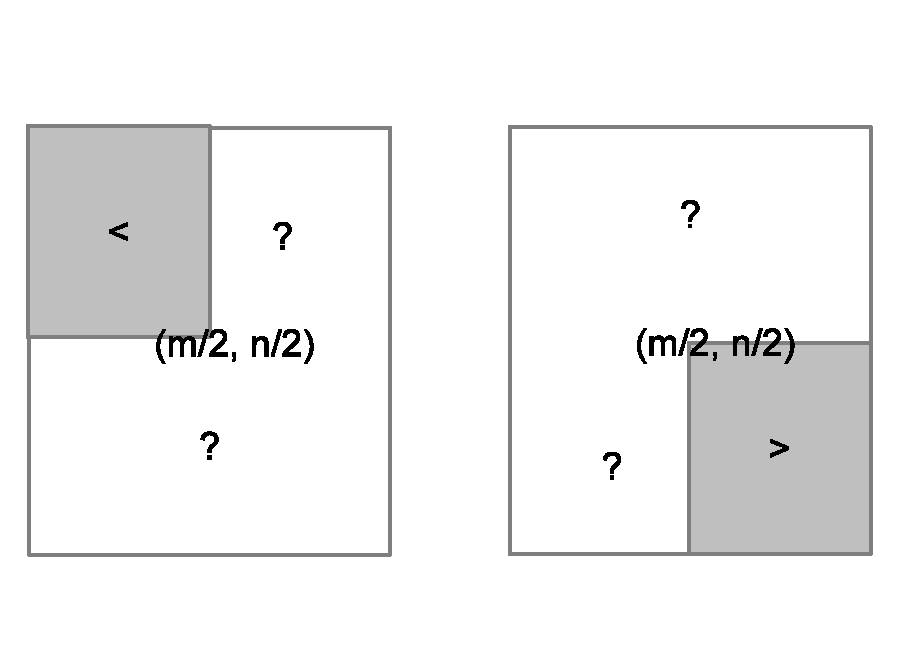
\includegraphics[scale=0.5]{img/bsearch-2D.eps}
 \caption{Left: the middle point element is smaller than $x$. All elements in the gray area are less than $x$; Right: the middle point element is greater than $x$. All elements in the gray area are greater than $x$.}
 \label{fig:bsearch-2D}
\end{figure}

The problem is that the solution domain chnages from a rectangle to a 'L' shape in both cases. We can't just
recursively apply search on it. In order to solve this problem systematically, we define the problem more
generally, use brute-force search as a start point, and keep improving it bit by bit.

Consider a function $f(x, y)$, which is strict increasing for its arguments, for instance $f(x, y) = a^x + b^y$, where
$a$ and $b$ are natural numbers. Given a value $z$, which is natural number as well. We want to sovle the equation
$f(x, y) = z$ by finding all candidate pairs $(x, y)$.

With this definition, the non-decreasing matrix search problem can be specialized by the below function. 

\[
f(x, y) = \left \{
  \begin{array}
  {r@{\quad:\quad}l}
  M_{x, y} & 1 \leq x \leq m, 1 \leq y \leq n \\
  -1 & otherwise
  \end{array}
\right.
\]

\paragraph{Brute-force 2D search}

As all solutions should be found for $f(x, y)$. One can immediately give the
brute force solution by embedded looping.

\begin{algorithmic}[1]
\Function{Solve}{$f, z$}
  \State $A \gets \Phi$
  \For{$x \in \{0, 1, 2, ..., z\}$}
    \For{$y \in \{0, 1, 2, ..., z\}$}
      \If{$f(x, y) = z$}
        \State $A \gets A \cup \{(x, y)\}$
      \EndIf
    \EndFor
  \EndFor
  \State \Return $A$
\EndFunction
\end{algorithmic}

This definately calculates $f$ for $(z+1)^2$ times. It can be formalized as in (\ref{eq:bsearch-brute}).

\be
solve(f, z) = \{ (x, y) | x \in \{0, 1, ..., z\}, y \in \{0, 1, ..., z\}, f(x, y) = z\}
\label{eq:bsearch-brute}
\ee

\paragraph{Saddleback search}

We haven't utilize the fact that $f(x, y)$ is strict increasing yet. Dijkstra pointed out in \cite{saddle-back}, instead
of searching from bottom-left corner, search from the top-left leads to a effective solution. As illustrated in figure 
\ref{fig:saddleback-1}, the search starts from $(0, z)$, for every point $(p, q)$, we compare $f(p, q)$ with $z$:

\begin{itemize}
\item If $f(p, q) < z$, since $f$ is strict increasing, for all $0 \leq y < q$, we have $f(p, y) < z$. We can drop all
points in the vertical line section (in red color); 
\item If $f(p, q) > z$, then $f(x, q) > z$ for all $p < x \leq z$. We can drop all points in the horizontal 
line section (in blue color); 
\item Otherwise if $f(p, q) = z$, we mark $(p, q)$ as one solution, then both line sections can be dropped. 
\end{itemize}

This is a systematical way to scale down the solution 
domain rectangle. We keep dropping either a row, or a column, or both. 

\begin{figure}[htbp]
 \centering
 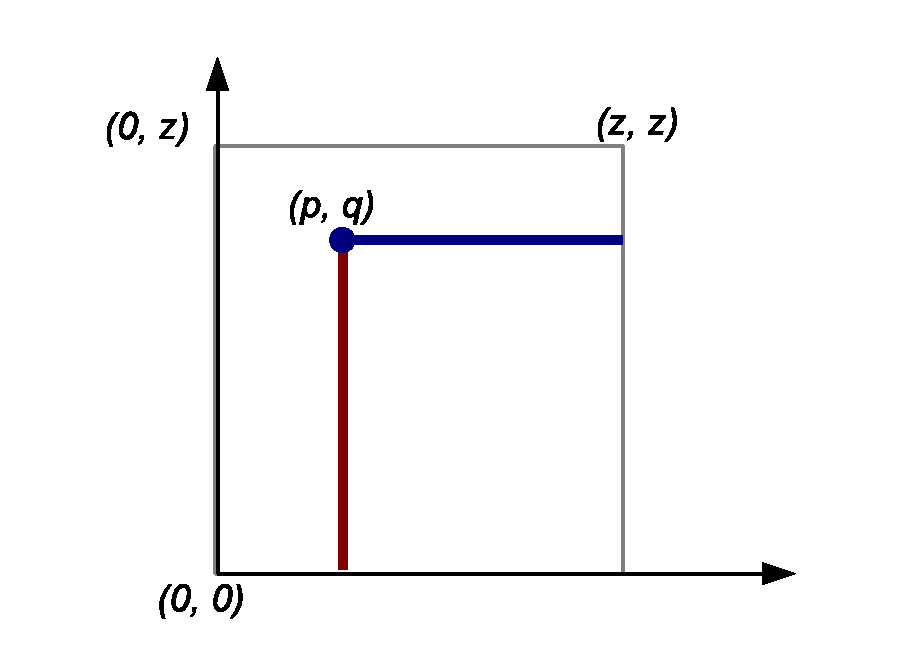
\includegraphics[scale=0.5]{img/saddleback-1.eps}
 \caption{Search from top-left.}
 \label{fig:saddleback-1}
\end{figure}

This method can be formalized as a function $search(f, z, p, q)$, which search solutions for equation $f(x, y) = z$ in
rectancle with top-left corner $(p, q)$, and bottom-right corner $(z, 0)$. We start the searching by intializing
$(p, q) = (0, z)$ as $solve(f, z) = search(f, z, 0, z)$

\be
search(f, z, p, q) =  \left \{
  \begin{array}
  {r@{\quad:\quad}l}
  \Phi & p > z \lor q < 0 \\
  search(f, z, p + 1, q) & f(p, q) < z \\
  search(f, z, p, q - 1) & f(p, q) > z \\
  \{(p, q)\} \cup search(f, z, p + 1, q - 1) & otherwise
  \end{array}
\right.
\ee

The first clause is the edge case, there is no solution if $(p, q)$ isn't on the top-left to $(z, 0)$. The following
example Haskell program implents this algorithm.

\lstset{language=Haskell}
\begin{lstlisting}
solve f z = search 0 z where
  search p q | p > z || q < 0 = []
             | z' < z = search (p + 1) q
             | z' > z = search p (q - 1)
             | otherwise = (p, q) : search (p + 1) (q - 1)
    where z' = f p q
\end{lstlisting}

Consider the calculation of $f$ is expensive, this program stores the result of $f(p, q)$ to variable $z'$.
This algorithm can also be implemented in iterative manner, that the boundaries of solution domain keeps being updated
in a loop.

\begin{algorithmic}[1]
\Function{Solve}{$f, z$}
  \State $p \gets 0, q \gets z$
  \State $S \gets \Phi$
  \While{$p \leq z \land q \geq 0$}
    \State $z' \gets f(p, q)$
    \If{$z' < z$}
      \State $p \gets p + 1$
    \ElsIf{$z' > z$}
      \State $q \gets q - 1$
    \Else
      \State $S \gets S \cup \{(p, q)\}$
      \State $p \gets p + 1, q \gets q - 1$
    \EndIf
  \EndWhile
  \State \Return $S$
\EndFunction
\end{algorithmic}

It's intuitive to translate this imperative algorithm to real program, for example, the following example Python code.

\lstset{language=Python}
\begin{lstlisting}
def solve(f, z):
    (p, q) = (0, z)
    res = []
    while p <= z and q >= 0:
        z1 = f(p, q)
        if z1 < z:
            p = p + 1
        elif z1 > z:
            q = q - 1
        else:
            res.append((p, q))
            (p, q) = (p + 1, q - 1)
    return res

\end{lstlisting}

It is clear that in every iteration, either $p$ or $q$ or both advance to the bottom-right corner by one.
Thus it takes at most $2(z+1)$ steps to complete searching. This is the worst case. There are three best
cases. The first one happens that in every iteration, both $p$ and $q$ advance by one, so that it needs 
only $z+1$ steps; The second case keeps advancing horizontally to right and ends when $p$ exceeds $z$;
The last case is similar, that it keeps moving down vertically to the bottom until $q$ becomes negative.

Figure \ref{fig:saddleback-1-cases} illustrates the bese cases and the worst cases respectively. Figure
\ref{fig:saddleback-1-cases} (a) is the case that every point $(x, z-x)$ in diagonal satisfies $f(x, z-x) = z$,
it uses $z+1$ steps to arrive at $(z, 0)$; (b) is the case that every point $(x, z)$ along the top
horizontal line gives the result $f(x, z) < z$, the algorithm takes $z+1$ steps to finish; (c) is
the case that every point $(0, x)$ along the left vertical line gives the result $f(0, x) > z$, thus
the algorithm takes $z+1$ steps to finish; (d) is the worst case. If we project all the horizontal
sections along the search path to $x$ axis, the project all the vertical sections to $y$ axis, it
gives the total steps of $2(z+1)$.

\begin{figure}[htbp]
 \centering
 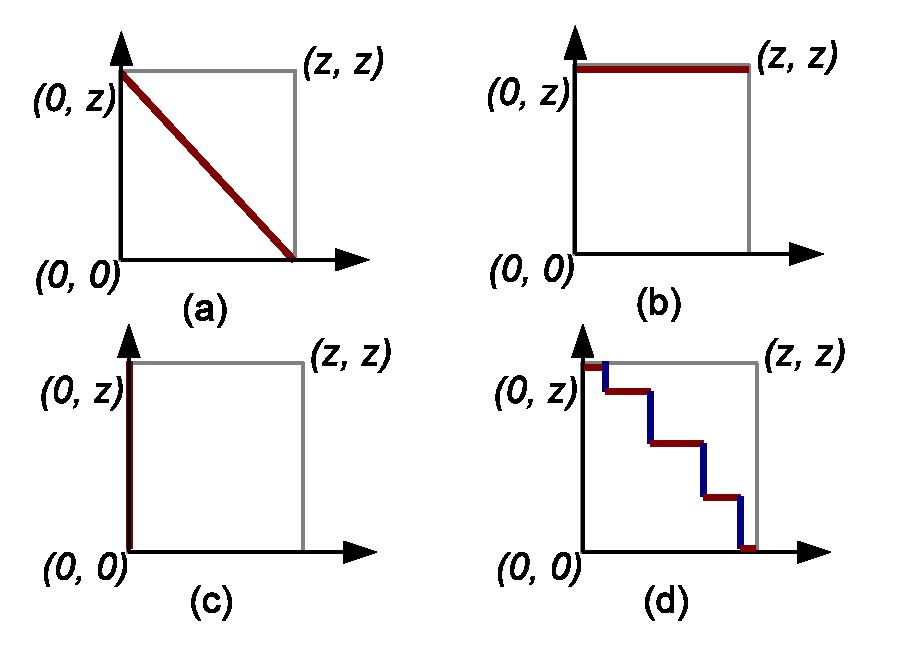
\includegraphics[scale=0.5]{img/saddleback-1-cases.eps}
 \caption{The best cases and the worst cases.}
 \label{fig:saddleback-1-cases}
\end{figure}

Compare to the quadratic brute-froce method ($O(z^2)$), we improve to a linear algorithm bound to $O(z)$.

TODO: the naming. 3-D plot

\paragraph{Improved saddleback search}

We haven't utilized the binary search tool so far, even the problem extends to 2-dimension domain.
The basic saddleback search starts from the top-left corner $(0, z)$ to the bottom-right corner $(z, 0)$.
This is acutally over-general domain. we can constrait it a bit more accurate.

Since $f$ is strict increasing, we can find the biggest number $m$, that $0 \leq m \leq z$, along the
$y$ axis which satisfies $f(0, m) \leq z$; Similarly, we can find the biggest $n$, that $0 \leq n \leq z$,
along the $x$ axis, which satisifes $f(n, 0) \leq z$; And the solution domain shrinks
from $(0, z) - (z, 0)$ to $(0, m) - (n, 0)$ as shown in figure \ref{fig:saddleback-2}.

\begin{figure}[htbp]
 \centering
 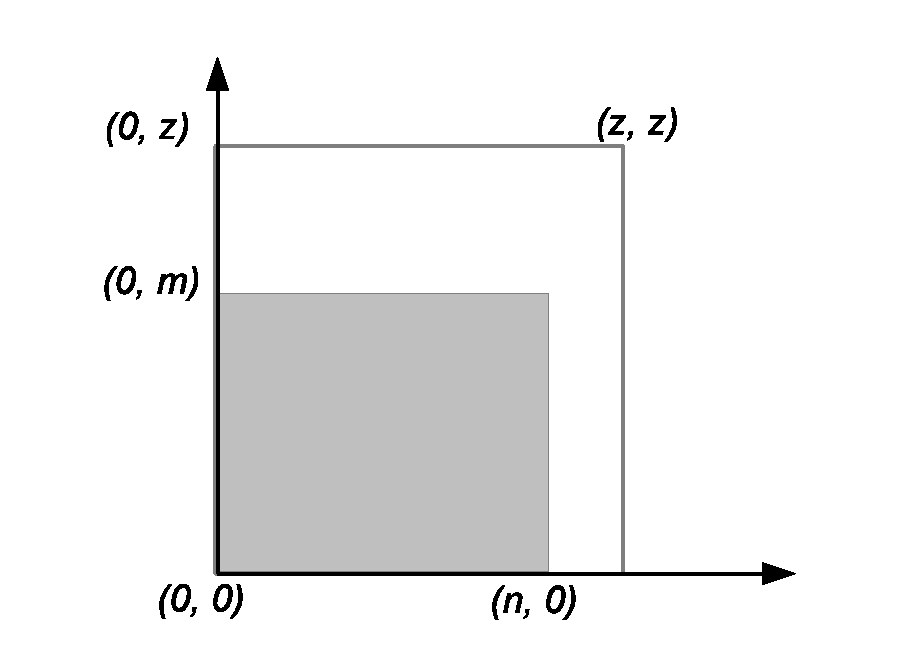
\includegraphics[scale=0.5]{img/saddleback-2.eps}
 \caption{A more accurate search domain shown in shaded color.}
 \label{fig:saddleback-2}
\end{figure}

Of course $m$ and $n$ can be found by brute-force searching like below.

\be
\begin{array}{rl}
m & = max(\{y | 0 \leq y \leq z, f(0, y) \leq z\}) \\
n & = max(\{x | 0 \leq x \leq z, f(x, 0) \leq z\})
\end{array}
\ee

When searching $m$, the $x$ variable of $f$ is bound to 0. It turns to be one dimension search problem
for a strict increasing function (or in functional term, a Curried function $f(0, y)$). Binary search works
in such case. However, we need a bit modification for equation (\ref{eq:bsearch}). Different from searching
a solution $l \leq x \leq u$, so that $f(x) = y$ for a given $y$; we need search for a solution
$l \leq x \leq u$ so that $f(x) \leq y < f(x+1)$.

\be
bsearch(f, y, l, u) = \left \{
  \begin{array}
  {r@{\quad:\quad}l}
  l & u \leq l \\
  m & f(m) \leq y < f(m+1), m = \lfloor \frac{l + u}{2} \rfloor \\
  bsearch(f, y, m + 1, u) & f(m) \leq y \\
  bsearch(f, y, l, m-1) & otherwise
  \end{array}
\right.
\label{eq:bsearch-general}
\ee

The first clause handles the edge case that the range contains less than one integer. The lower
boundary is returned in such case;
If the middle point produces a value less than or equal to the target, while the next one evaluates
to a bigger value, the middle point is what we are looking for;
Otherwise if the point next to the middle also evaluates to a value not greater than the target,
the lower bound is increased by one, and we perform recursively binary search;
The only left case is that, the middle point evaluates to a value greater than the target,
upperbound is updated as the point preceeds to the middle for furthur recursive searching. The following
Haskell example code implements this modified binary search.

\lstset{language=Haskell}
\begin{lstlisting}
bsearch f y (l, u) | u <= l = l
                   | f m <= y = if f (m + 1) <= y then bsearch f y (m + 1, u) else m
                   | otherwise = bsearch f y (l, m-1)
  where m = (l + u) `div` 2
\end{lstlisting}

Then $m$ and $n$ can be found by using this binary search function.

\be
\begin{array}{rl}
m & = bsearch(\lambda_y \cdot f(0, y), z, 0, z) \\
n & = bsearch(\lambda_x \cdot f(x, 0), z, 0, z)
\end{array}
\label{eq:bsearch-boundaries}
\ee

And the improved saddleback search shrinks to this new search domain $solve(f, z) = search(f, z, 0, m)$:

\be
search(f, z, p, q) =  \left \{
  \begin{array}
  {r@{\quad:\quad}l}
  \Phi & p > n \lor q < 0 \\
  search(f, z, p + 1, q) & f(p, q) < z \\
  search(f, z, p, q - 1) & f(p, q) > z \\
  \{(p, q)\} \cup search(f, z, p + 1, q - 1) & otherwise
  \end{array}
\right.
\ee

It's almost as same as the basic saddleback version, except that it stops if $p$ exceeds $n$, but not $z$.
In real implementation, the result of $f(p, q)$ can be calculated once, and stored in a variable as
shown in the following Haskell example.

\lstset{language=Haskell}
\begin{lstlisting}
solve' f z = search 0 m where
  search p q | p > n || q < 0 = []
             | z' < z = search (p + 1) q
             | z' > z = search p (q - 1)
             | otherwise = (p, q) : search (p + 1) (q - 1)
    where z' = f p q
  m = bsearch (f 0) z (0, z)
  n = bsearch (\x->f x 0) z (0, z)
\end{lstlisting}

This improved saddleback firstly performs binary search two rounds to find the proper $m$, and $n$.
Eash round is bound to $O(\lg z)$ times of calculation for $f$; After that, it takes $O(m + n)$
time in the worst case; and $O(min(m, n))$ time in the best case. The overall performance is
given in the following table.

\begin{tabular}{|l|l|}
\hline
 & times of evaluation $f$ \\
\hline
worst case & $2 \log z + m + n$ \\
best case & $2 \log z + min(m, n)$ \\
\hline
\end{tabular}

For some function $f(x, y) = a^x + b^y$, for positive integers $a$ and $b$, $m$ and $n$ will be
relative small, that the performance is near to $O(\lg z)$.

This algorithm can also be realized in imperative approach. Firstly, the binary search should be modified.

\begin{algorithmic}[1]
\Function{Binary-Search}{$f, y, (l, u)$}
  \While{$l < u$}
    \State $m \gets \lfloor \frac{l + u}{2} \rfloor$
    \If{$f(m) \leq y$}
      \If{$y < f(m+1)$}
        \State \Return m
      \EndIf
      \State $l \gets m + 1$
    \Else
      \State $u \gets m$
    \EndIf
  \EndWhile
  \State \Return $l$
\EndFunction
\end{algorithmic}

Utilize this algorithm, the boundaries $m$ and $n$ can be found before performing the saddleback search.

\begin{algorithmic}[1]
\Function{Solve}{$f, z$}
  \State $m \gets$ \Call{Binary-Search}{$\lambda_y \cdot f(0, y), z, (0, z)$}
  \State $n \gets$ \Call{Binary-Search}{$\lambda_x \cdot f(x, 0), z, (0, z)$}
  \State $p \gets 0, q \gets m$
  \State $S \gets \Phi$
  \While{$p \leq n \land q \geq 0$}
    \State $z' \gets f(p, q)$
    \If{$z' < z$}
      \State $p \gets p + 1$
    \ElsIf{$z' > z$}
      \State $q \gets q - 1$
    \Else
      \State $S \gets S \cup \{(p, q)\}$
      \State $p \gets p + 1, q \gets q - 1$
    \EndIf
  \EndWhile
  \State \Return $S$
\EndFunction
\end{algorithmic}

The implementation is left as exercise to the reader.

\paragraph{More improvement to saddleback search}

In figure \ref{bsearch-2D}, two cases are shown for comparing the value of the middle point in a matirx with the given value.
One case is the center value is smaller than the given value, the other is bigger. In both case, we can only throw away
$\frac{1}{4}$ candidates, and left a 'L' shape for further searching.

Actually, one important case is missing. We can extend the observation to any point inside the rectagle searching area.
As shown in the figure \ref{fig:saddleback-drop}.

\begin{figure}[htbp]
 \centering
 \subfloat[If $f(p, q) \neq z$, only lower-left or upper-right sub area (in gray color) can be thrown. Both left a 'L' shape.]{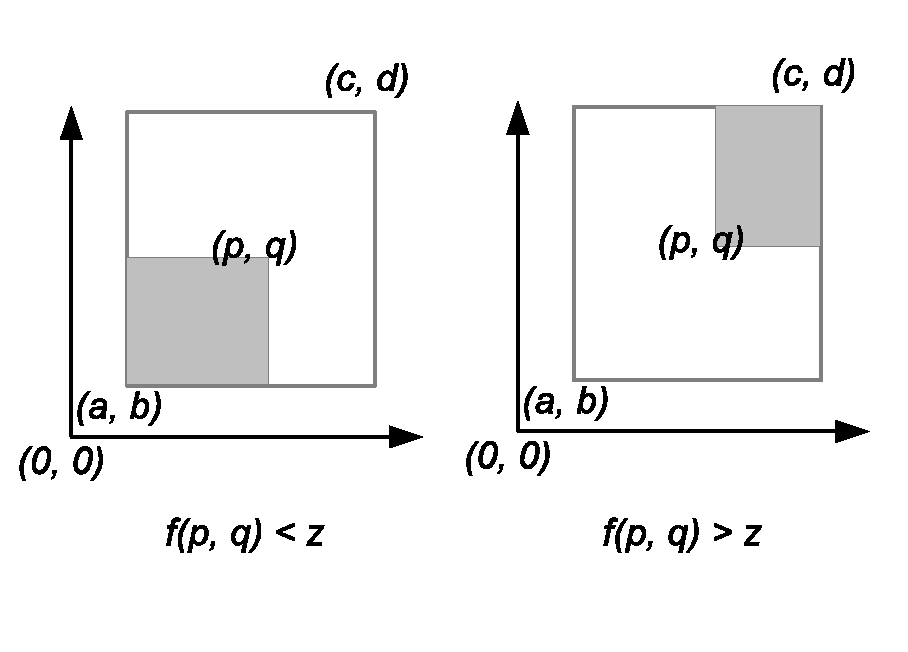
\includegraphics[scale=0.5]{img/saddleback-3.eps}} \\
 \subfloat[If $f(p, q) = z$, both sub areas can be thrown, the scale of the problem is halved.]{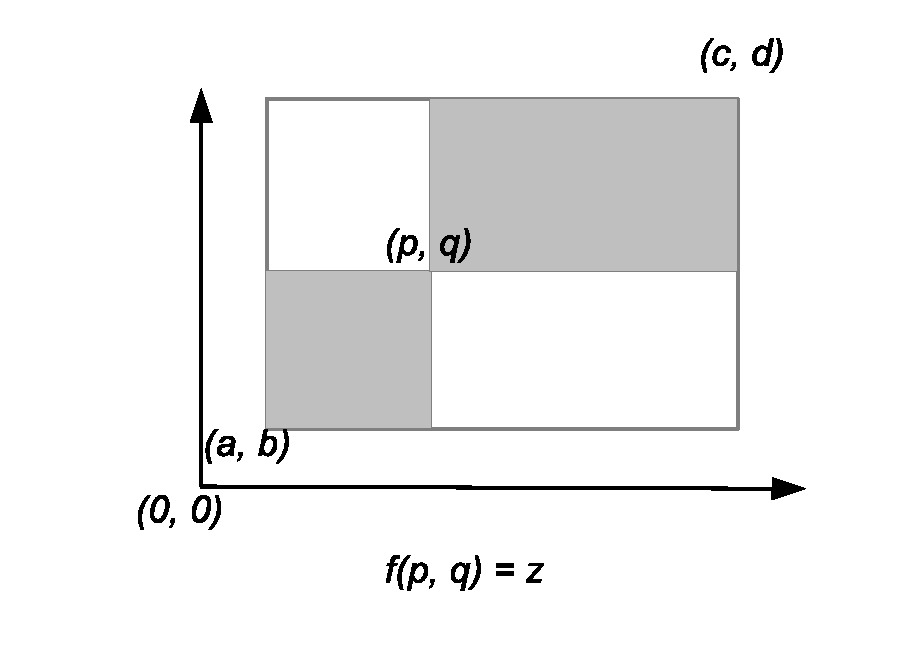
\includegraphics[scale=0.5]{img/saddleback-4.eps}}
 \caption{The efficiency of scaling down the search domain.}
 \label{fig:saddleback-drop}
\end{figure}

Suppose we are searching in a rectangle from the lower-left corner $(a, b)$ to the upper-right corner $(c, d)$.
If the $(p, q)$ isn't the middle point, and $f(p, q) \neq z$. We can't ensure the area to be dropped is always
1/4. However, if $f(p, q) = z$, as $f$ is strict increasing, we are not only sure both the lower-left and the
upper-right sub areas can be thrown, but also all the other points in the column $p$ and row $q$. The problem
can be scaled down fast, because only 1/2 area is left.

This indicates us, instead of jumping to the middle point to start searching. A more efficient way is to find
a point which evaluates to the target value. One straightforward way to find such a point, is to perform
binary search along the center horizontal line or the center vertical line of the rectangle.

The performance of binary search along a line is the length of that line. A good idea is alway pick the shorter
center line as shown in figure \ref{fig:saddleback-centerline}. That if the height of the rectangle is longer
than the width, we perform binary search along the horizontal center line; otherwise we choose the vertical
center line.

\begin{figure}[htbp]
 \centering
 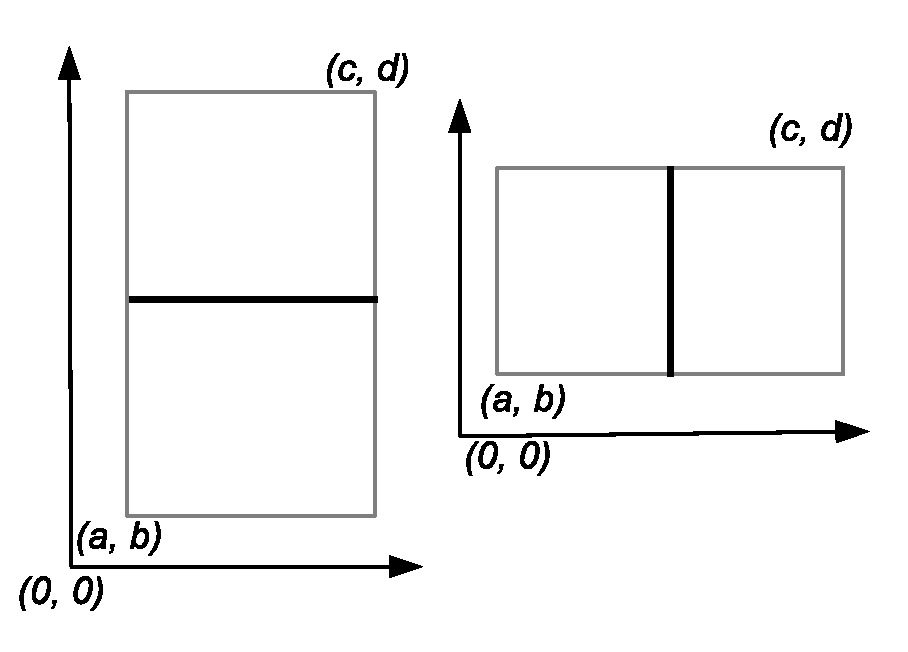
\includegraphics[scale=0.5]{img/saddleback-centerline.eps}
 \caption{Binary search along the shorter center line.}
 \label{fig:saddleback-centerline}
\end{figure}

However, what if we can't find a point $(p, q)$ in the center line, that satisfies $f(p, q) = z$? Let's take
the center horizontal line for example. even in such case, we can still search for a point that
$f(p, q) < z < f(p+1, q)$. The only difference is that we can't drop the points in row $p$ and $q$ completely.

Combine this condition, the binary search along the horinzontal line is to find a $p$, satisifies 
$f(p, q) \leq z < f(p+1, q)$; While the vertical line search condition is $f(p, q) \leq z < f(p, q + 1)$.

The modified binary serach ensures that, if all points in the line segment give $f(p, q) < z$, the upper
bound will be found; and the lower bound will be found if they all greater than $z$. We can drop the
whole area on one side of the center line in such case.

Sum up all the ideas, we can develop a effcient improved saddleback search as the following.

\begin{enumerate}
\item Perform binary search along the $y$ axis and $x$ axis to find the tight boundaries from $(0, m)$ to $(n, 0)$;
\item Denote the candidate rectangle as $(a, b) - (c, d)$, if the candidate rectangle is empty, the solution is empty;
\item If the height of the rectangle is longer than the width, perform binary search along the center horinzontal line; otherwise, perform binary search along the center vertical line; denote the search result as $(p, q)$;
\item If $f(p, q) = z$, record $(p, q)$ as a solution, and recursively search two sub rectangles $(a, b) - (p-1, q+1)$ and
$(p+1, q-1) - (c, d)$;
\item Otherwise, $f(p, q) \neq z$, recursively the same two sub rectangles plus a line section. The line section
is either $(p, q+1) - (p, b)$ for center vertical line; or $(p+1, q) - (c, q)$ for center horizontal line.
\end{enumerate}

Figure \ref{fig:include-line} shows the line section should be included for recursively search.

\begin{figure}[htbp]
 \centering
 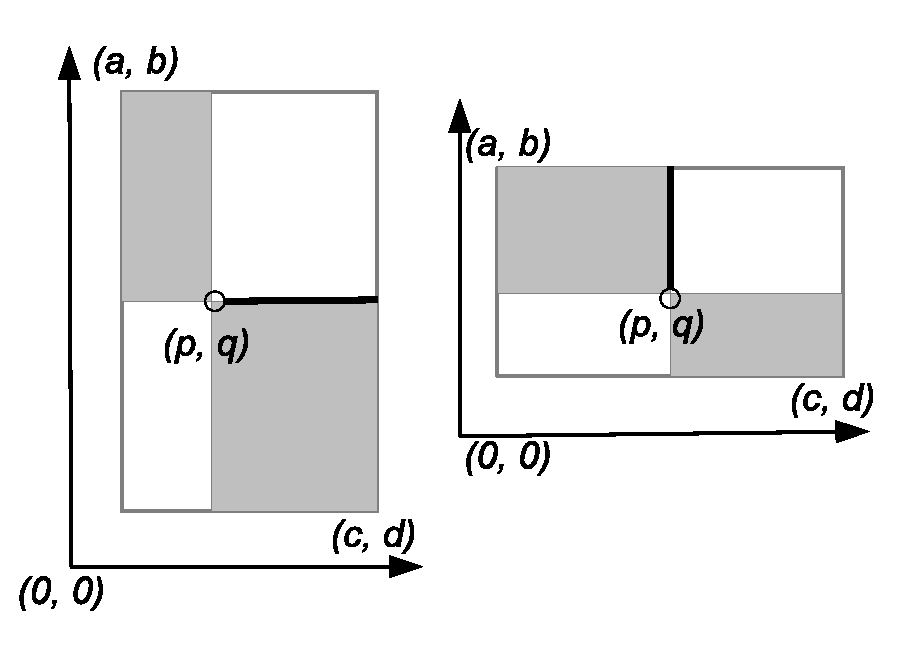
\includegraphics[scale=0.5]{img/saddleback-include-ln.eps}
 \caption{Recursively search the gray areas, the bold line should be included if $f(p, q) \neq z$.}
 \label{fig:include-line}
\end{figure}

This algorithm can be formalized as the following. The equation (\ref{eq:bsearch-general}), and (\ref{eq:bsearch-boundaries})
are as same as before. A new $search$ function should be defined.

\be
search(f, z, (a, b), (c, d)) =  \left \{
  \begin{array}
  {r@{\quad:\quad}l}
  \Phi & c < a \lor d < b \\
  csearch(f, z, (a, b), (c, d)) & c - a < d - b \\
  rsearch(f, z, (a, b), (c, d)) & otherwise
  \end{array}
\right.
\ee

\begin{Exercise}
\begin{itemize}
\item Prove that the average case of the divide and conquer solution to $k$-selection problem is $O(n)$. Please refer to previous chapter about quick sort.
\item Implement the imperative $k$-selection problem with 2-way partition, and median-of-three pivot selection.
\item Implement the imperative $k$-selection problem to handle duplicated elements effectively.
\item Realize the median-of-median $k$-selection algorithm and implement it in your favorite programming language.
\item The $tops(k, L)$ algorithm uses list concatenation likes $A \cup \{ l_1 \} \cup tops(k - |A| - 1, B)$. It is linear operation which is proportion to the length of the list to be concatenated. Modify the algorithm so that the sub lists are concatenated by one pass.
\item The author considered another divide and conquer solution for the $k$-selection problem. It finds the maximum of the
first $k$ elements and the minimum of the rest. Denote them as $x$, and $y$. If $x$ is smaller than $y$, it means that 
all the first $k$ elements are smaller than the rest, so that they are exactly the top $k$ smallest; Otherwise, There
some elements in the first $k$ should be moved.
\begin{algorithmic}
\Procedure{Tops}{$k, A$}
  \State $l \gets 1$
  \State $u \gets |A|$
  \Loop
    \State $i \gets$ \Call{Max-At}{$A[l..k]$}
    \State $j \gets$ \Call{Min-At}{$A[k+1..u]$}
    \If{$A[i] < A[j]$}
      \State break
    \EndIf
    \State \textproc{Exchange} $A[l] \leftrightarrow A[j]$
    \State \textproc{Exchange} $A[k+1] \leftrightarrow A[i]$
    \State $l \gets$ \Call{Partition}{$A, l, k$}
    \State $u \gets$ \Call{Partition}{$A, k+1, u$}
  \EndLoop
\EndProcedure
\end{algorithmic}
Explain why this algorithm works? What's the performance of it?
\item Implement the binary search algorithm in both recursive and iterative manner, and try to verify your version
automatically. You can generate randomized data, test your program with the binary search invariant and against the
one provided in your standard library.
\item Implement the improved saddleback search by first performing binary search to find a more accurate solution domain
in your favorite imperative programming language.
\end{itemize}
\end{Exercise}

\subsection{Information reuse}

\subsubsection{Boyer-Moore majority number}

\subsubsection{KMP}

\subsubsection{Boyer-moore}

\section{Solution searching}
\subsection{DFS and BFS}

\subsection{Search the optimal solution}

\subsection{Dynamic programming}

\subsection{Grady algorithm}

\section{Short summary} 
summary

\begin{thebibliography}{99}

\bibitem{TAOCP}
Donald E. Knuth. ``The Art of Computer Programming, Volume 3: Sorting and Searching (2nd Edition)''. Addison-Wesley Professional; 2 edition (May 4, 1998) ISBN-10: 0201896850 ISBN-13: 978-0201896855

\bibitem{CLRS}
Thomas H. Cormen, Charles E. Leiserson, Ronald L. Rivest and Clifford Stein. 
``Introduction to Algorithms, Second Edition''. ISBN:0262032937. The MIT Press. 2001

\bibitem{median-of-median}
M. Blum, R.W. Floyd, V. Pratt, R. Rivest and R. Tarjan, "Time bounds for selection," J. Comput. System Sci. 7 (1973) 448-461.

\bibitem{programming-pearls}
Jon Bentley. ``Programming pearls, Second Edition''. Addison-Wesley Professional; 1999. ISBN-13: 978-0201657883

\bibitem{fp-pearls}
Richard Bird. ``Pearls of functional algorithm design''. Cambridge University Press. 2010. ISBN, 1139490605, 9781139490603

\bibitem{saddle-back}
Edsger W. Dijkstra. ``The saddleback search''. EWD-934. 1985. http://www.cs.utexas.edu/users/EWD/index09xx.html.

\end{thebibliography}

\ifx\wholebook\relax\else
\end{document}
\fi

